\chapter{Parking}
\label{ch:parking}
% ##################################################################################################################

\hfill \textbf{Author:} Rashid A. Waraich

\begin{center} 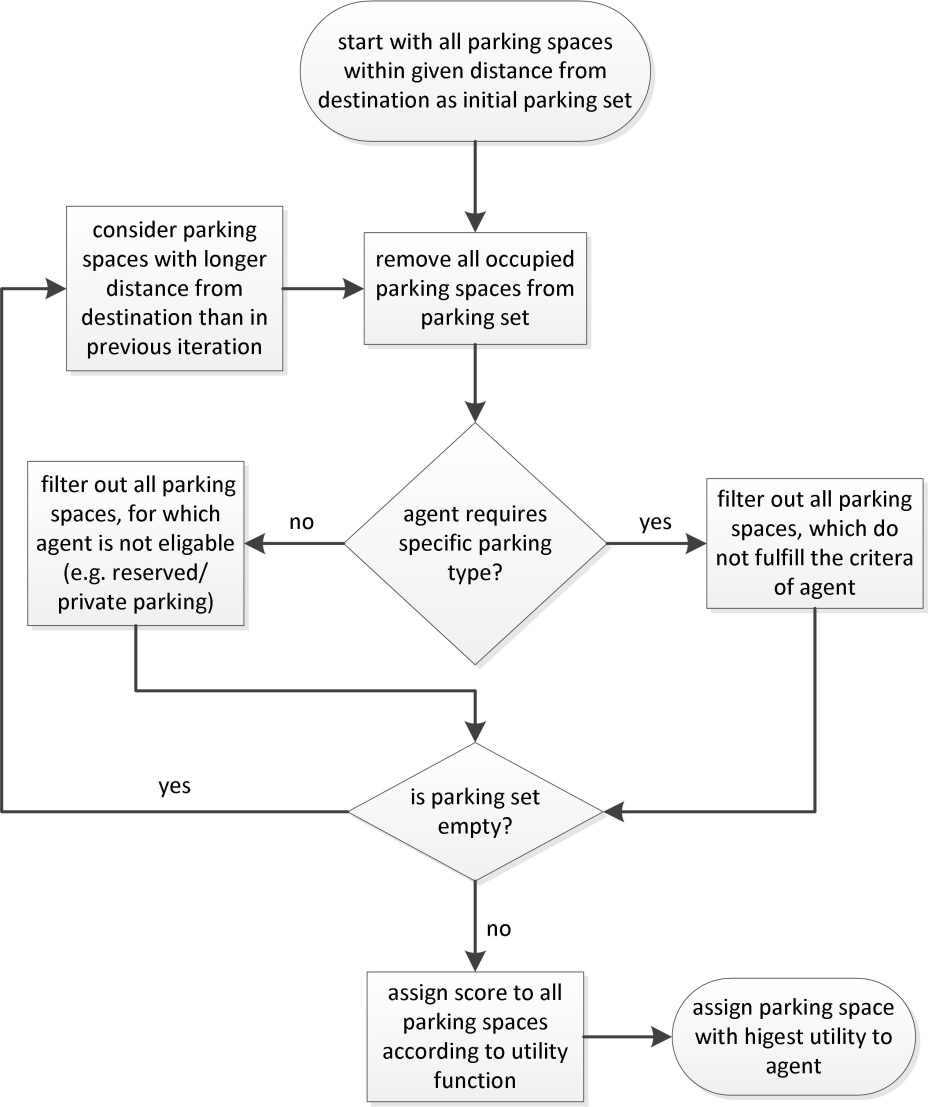
\includegraphics[width=0.4\textwidth, angle=0]{extending/figures/Parking/parking_algo.png} \end{center}

\createStandardInformation{parking}{todo}{todo}{\citet[][]{WaraichAxhausen_TRR_2012, WaraichEtAl_TechRep_IVT_2012, WaraichAxhausen_TechRep_IVT_2012, WaraichEtAl_TechRep_IVT_2013_2, Waraich_unpub_Brownbag_2014, WaraichEtAl_unpub_STRC_2014}}

% ##################################################################################################################
\section{Introduction} 
The \gls{matsim} simulation by default does not consider parking infrastructure or supply constraints. This however can lead to too high car vehicle traffic to city centers in the model, which are often not present in the real-world due to limited parking. Modeling parking is also important as traffic related policies can be designed around parking. E.g. raising the prices for parking at certain times of the day or reducing parking supply in an area can impact travel demand. 

This chapter describes some of the work related to parking models for \gls{matsim}, which has tried to bridge this gap.

% ##################################################################################################################
\section{Models}
For technical reasons, the modeling efforts around parking in \gls{matsim} are divided in two parts parking choice and parking search, which are described in the following two subsections. 

% ==================================================================================
\subsection{Parking Choice Model}
The first approach for modeling does not change the \gls{matsim} traffic simulation, but only extends it to capture parking supply by means of controller listeners and event handling. This means there is no rerouting happening during the simulation due to parking. However changed routes can be incorporated in a post-processing step, as described in \citet[][]{WaraichAxhausen_TRR_2012}. 

In the most general case, a parking choice model performs the following simulation steps: At the time of arrival of a vehicle at a destination in \gls{matsim}, the parking choice model assigns a parking in the surroundings to the agent according to a customizable algorithm (e.g.,\,utility maximization). The assigned parking is marked as occupied on arrival and becomes unoccupied again, when the agent departs. In this way the model simulates supply side constraints with the same temporal resolution as the basic \gls{matsim} model.

A simple version of the parking choice model can just consider walk distance minimization and ignore other user preferences and park at the closest available public parking. Already such a simple model is able to partly solve one of the main problems of the un-constraint parking model in \gls{matsim}, as it makes an area with little parking less attractive for traveling to with car due to longer walk distances. The integration of the parking model with \gls{matsim} is achieved by adding a term for the parking operation to the overall agent’s plan scoring function, where this term looks as follows.

\begin{equation}
\label{eq:parkingutf}
S_{parking} = S_{walking} + S_{parking\ costs} + S_{parking\ search\ time}
\end{equation}

Beyond walking distance disutility, this scoring function can also include additional features like cost or even estimated parking search times, e.g. using models like presented in \citet[][]{HorniEtAl_IATBRspec_2013}.

A study for the city of Zürich, which implements a parking choice model and includes trade-off between walk distance and parking cost is presented in \citet[][]{WaraichAxhausen_TRR_2012}. Moreover in this study also the distinction between public, private and reserved parking is made, where only certain people (e.g.,\,disabled) or certain vehicles can park (e.g.,\,electric vehicles). Figure~\ref{fig:parkingchoicealgo} shows the parking choice model employed in this study, where a distinction between public, private and reserved parking is made. In \citet[][]{WaraichEtAl_unpub_TRB_2013} another study for modeling parking in \gls{matsim} is reported, where individual preferences with regards to parking in terms of gender and age are considered. The utility function parameters used in this study are estimated based on a stated preference survey in Switzerland.

 % ------------
\createfigure%
{Parking choice algorithm}%
{Parking choice algorithm}%
{\label{fig:parkingchoicealgo}}%
{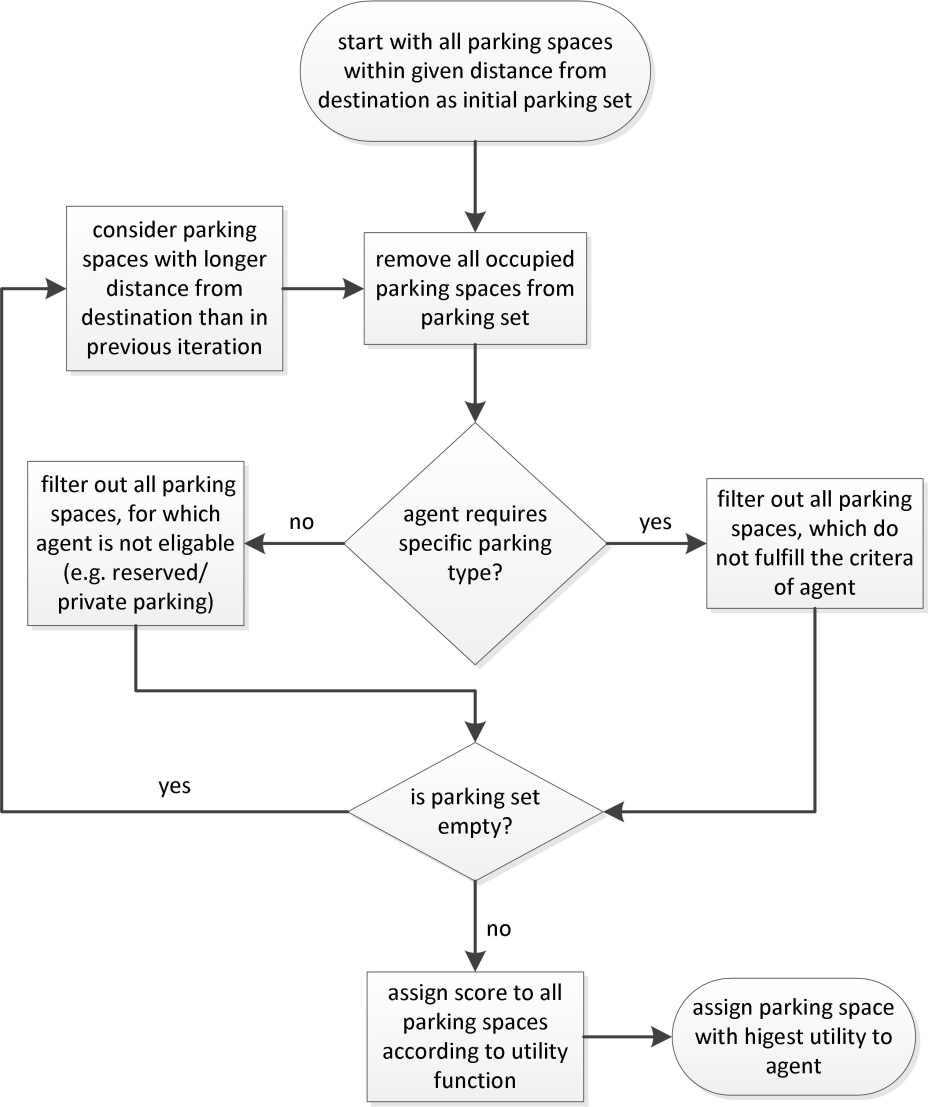
\includegraphics[width=0.8\textwidth, angle=0]{extending/figures/Parking/parking_algo.png}}%
{\citet[][]{WaraichAxhausen_TRR_2012}}
% ------------

% ==================================================================================
\subsection{Parking Search}
The parking choice model presented in the previous section is able to capture many relevant aspects of parking. However, it does not model parking search behavior. Some studies conducted around the globe suggest that on average around 30\,\% of the traffic at city centers could be due to parking search traffic \citet[][]{Shoup_RSUE_2004}. Therefore it seems important to capture parking search related traffic in transportation models.

A first idea to model parking search traffic in \gls{matsim} is presented in \citet[][]{Waraich_unpub_IATBR_2012}. The basic idea comes from surveys, which suggest that people select certain strategies when starting the parking search process, which they think will be beneficial for them \citet[][]{AxhausenPolak_1989}. While a proof of concept was attempted for development using within-day replanning (see Chapter~\ref{ch:withinday}, \citep[][]{DoblerEtAl_TRR_2012}), this path was aborted after development of a couple of initial strategies, where especially performance and integration issues lead to a dead-end \citet[][]{WaraichEtAl_unpub_TRB_2013}---performance after optimization around 24\,times slower than for the original runs without parking operations. 

We have now successfully perused an alternative path towards the idea presented in \citet[][]{Waraich_unpub_IATBR_2012} by implementing a \gls{jdeqsim} based model (see Section~\ref{sec:jdeqsim}) with within-day support and approximation of travel times like in PSim (see Chapter~\ref{ch:psim}, \citet[][]{FourieEtAl_TRR_2013}). This removes the overhead, which was present in the previous approach and gave us the flexibility to implement many of the parking strategies presented in \citet[][]{AxhausenPolak_1989} and beyond. First results of this approach are planned to be published in 2015.

% ##################################################################################################################
\section{Applications}
Obviously, applications of the presented parking models are many-fold and especially well-suited for policy design. E.g.,\,an example of traffic policy design by means of targeted reduction of parking supply is presented in \citet[][]{WaraichAxhausen_TRR_2012}. In \citet[][]{WaraichEtAl_unpub_TRB_2013} an application of performance-based pricing for parking in \gls{matsim} is shown, where iteratively parking prices are adapted to match demand. An integration of parking choice and electric vehicle charging is presented in \citet[][]{WaraichEtAl_JanssensEtAl_2014} for a case study in Zürich. An even more sophisticated test model for parking and electric vehicle charging is presented in \citet[][]{BemezHohenfeller_BSCThesis_2014}, where various types of charging speed and prices are present.

% ##################################################################################################################
\section{Usage}
A general parking choice models is included in the parking contribution of \gls{matsim}, which provides various interfaces for extension. Furthermore examples are included in the parking contribution, in order to provide guidance for extension. 

% ##################################################################################################################


